\documentclass{article}

\usepackage{amsmath, amssymb, amsthm}
\usepackage{tikz}
\usepackage{tikz-uml}
\usepackage{graphicx}

\title{Girth}
\author{Christiaan van de Sande}

\renewcommand*{\theenumi}{\thesubsection.\arabic{enumi}}
\renewcommand*{\theenumii}{\theenumi.\arabic{enumii}}
\newenvironment{changemargin}[2]{%
  \begin{list}{}{%
    \setlength{\topsep}{0pt}%
    \setlength{\leftmargin}{#1}%
    \setlength{\rightmargin}{#2}%
    \setlength{\listparindent}{\parindent}%
    \setlength{\itemindent}{\parindent}%
    \setlength{\parsep}{\parskip}%
  }%
\item[]}{\end{list}}

\begin{document}
\maketitle

\section{Introduction}

Girth is a program that allows the user to create and manipulate graphs (mathematical objects with vertices and edges).
It was inspired by a concurrent enrollment in MAT 416 (Graph Theory),
where many of the graphs being studied are too big to draw by hand and hard to visualize without a picture.
For these graphs, a computer-generated picture can be very useful.

Now the initially created drawing might not be the most helpful, and different drawings might be ideal for different purposes.
To address this need, the user should be able to move the vertices of the graph and manipulate the drawing as desired.

Beyond simply seeing the graphs, there are several properties of graphs that are impractical to calculate by hand,
but much easier to find using simple algorithms. These include girth, diameter, and clique number.

What follows is a brief overview of Girth,
including the requirements for the project
and intricate details about the design of the program and the process by which it came about.

\section{Requirements}

\subsection{Graphical Interface}
\begin{enumerate}
  \item The interface should be clean and attractive.
  \item The interface should be simple and intuitive.
  \item The interface should be complete - all necessary tools should be easy to find and use
        and relevant information (i.e. errors and other status information) should be clearly displayed.
\end{enumerate}

\subsection{Functionality}
\begin{enumerate}
  \item Method return values must be faithful to the mathematical defenitions (e.g. Graph.getGirth must return the girth)
  \item Constructors and methods must not be able to create an invalid graph.
  \item The program must be capable of representing any graph $ G $ with $ | G |, \| G \| < N $ where $ N $ is java's
        maximum integer value.
\end{enumerate}

\subsection{Implementation}
\begin{enumerate}
  \item The graphical interface must be implemented using javafx without any outside dependencies or usage of the depreciated
        swing package.
  \item The program must be written entirely in java and javafx without any outside dependencies.
\end{enumerate}

\section{Approach}

The centerpiece of Girth is the Graph class, so most of the project time was devoted to developing that class.
The Graph class was designed, created, and tested before any other development of the program.
After the Graph class was proven by numerous test cases, the GUI portion was planned and implemented.
Finally, the program was refined in its entirety to eliminate bugs and add features.

The code for the project was written entirely by the author
with helpful advice from some classmates and friends.
Stack Overflow and Oracle were utilized throughout the development process,
and some of the algorithms were partially sourced by Math Stack Exchange.

\section{Design}

There are many ways of simulating graphs in code.
For example,
the vertices can be thought of as objects that link to other vertices much like nodes in a linked list - the neighborhoods method;
the edges can be thought of as objects that each have a pair of vertices - the edge set method;
or the edges can be encoded in a two dimensional array where the vertices are indices - the adjacency matrix method.

Each of these mthods has its advantages and disadvantages.
The neighborhoods and edge-set methods are most efficient for sparce graphs (graphs with many vertices and very few edges),
while the adjacency-matrix method is does not experience as much variation from the number of edges.
For Girth, the adjacency-matrix method was used.

After determining the representation of the graph, the next question to answer is what kinds of graphs to allow.
Simple graphs (Graphs with no vertices adjacent to themselves, at most one edge per pair of vertices, and every edge going both ways)
are by far the most studied and must be represented.
However multigraphs (where multiple edges can exist between the same vertices),
directed graphs (where the edges have a particular orientation),
and pseudographs (where some vertices may have edges to themselves),
are also occasionally studied.

Girth was designed primarily to handle simple graphs and,
while the underlying Graph class supports pseudographs and directed graphs,
only simple graphs are supported by the graphical interface.
The Graph class also supports weighted edges, which the graphical interface does not yet incorperate. 

\subsection{Layout}

Below is a picture of the Girth GUI.
On the right, titled "Graph Details" is the QueryPane, which displays information about the current graph.
On the bottom, the Graph Builder is shown with the parameters set up to generate the Generalized Peterson Graph for 5, 4.
In the center, the DrawingPane depicts the Generalized Peterson 5, 4 graph with an added vertex
(shown in the upper right corner).
Vertices are shown in blue, selected Vertices are colored red.

\begin{center}\includegraphics[width=4in, keepaspectratio]{pictures/add-vertex.png}\end{center}

\subsection{Classes}

Girth is designed to be highly modular. The classes are highly independent and can be used in a variety of configurations.

\subsubsection{Graph}

The Graph class is the heart of the program.
It is designed to be entirely independent of the rest of the program
and functional as a stand-alone tool for creating and interacting with graphs.
Its capabilities go well beyond those availible to the Girth GUI and the requirements of project.
Fully utilizing the Graph class would require a much more elaborate program.

\subsubsection{ArrayIndexOrdering}

ArrayIndexOrdering is a Comparator that uses an array of comparable values to compare indices.
In the context of Girth,
ArrayIndexOrdering is used in the distance algorithm to sort vertices by their distance from a particular root vertex.
The ArrayIndexOrdering class implements the Comparator interface.

\subsubsection{GraphWrapper}

The GraphWrapper class handles the interactions between the GUI components and the Graph.
Mainly, it exists to ensure that the components of the UI are updated when the graph is alterred.
The GraphWrapper also allows the Graph to be exchanged without replacing the its reference in the entire program.

\subsubsection{Vertex}

The Vertex class contains the information that is needed for each vertex.
Configurations of the program that require additional information about the vertices would require a rewrite of this class,
which is a notable weakness of the programs design. 

\subsubsection{Listener}

The Listener interface defines the methods needed for components that need to be updated when the graph is alterred
or a new graph is created.

\subsubsection{DrawingPane}

The DrawingPane class is the primary GUI component. This class is responsible for generating a drawing of the graph
that allows the user to move, select, and deselect vertices.
The DrawingPane class extends the Canvas class and implements the Listener interface.

\subsubsection{BuildPane}

The BuildPane class provides a tool for creating graphs as well as adding and deleting vertices.
The BuildPane class extends the VBox class.

\subsubsection{QueryPane}

The QueryPane class displays details about the graph. This class does not provide any access to manipulating the graph.
The QueryPane class extends the VBox class and implements the Listender interface.\\

The DrawingPane, BuildPane, and QueryPane classes are completely modular independent from each other.
Although they all depend on the Vertex and GraphWrapper classes.

\subsubsection{Girth}

The Girth class is the main application class of the program.
Most of the functionality is controlled by other classes,
so the Girth class is free to act as a configurator for the program.
The Girth class extends the Application class.

\subsection{UML Diagram}
\begin{changemargin}{-1in}{-1in}
\begin{center}
\begin{tikzpicture}
\umlsimpleclass[x=-1]{Girth}
\umlclass[x=2, y=-2.5]{BuildPane}{
  - graphWrapper: GraphWrapper \\
  - state: String \\
  - warning: Label \\
  - input: TextField}{}
\umlclass[x=2, y=-5.5]{QueryPane}{
  - graphWrapper: GraphWrapper \\
  - results: Label}{
  + update() : void \\ + initialize() : void}
\umlclass[x=2, y=-11]{DrawingPane}{
  - graphWrapper: GraphWrapper \\
  - state: String \\
  - dragVertex: Vertex \\
  - dragging: boolean \\
  - LINE\_WIDTH: double \\
  - VERTEX\_RADIUS: double \\
  - EDGE\_COLOR: Color \\
  - SELECTED\_COLOR: Color \\
  - VERTEX\_COLOR: Color}{
  + update() : void \\ + initialize() : void}

\umlclass[type=interface,x=-3, y=-7.5]{Listener}{}{+ update() : void \\ + initialize() : void}

\umlclass[x=9, y=-3]{GraphWrapper}{
  - graph: Graph \textlangle Vertex\textrangle \\
  - listeners: ArrayListListeners}{
  + setGraph(Graph g): void \\
  + getGraph(): Graph \textlangle Vertex\textrangle \\
  + update(): void \\
  + initialize(): void \\
  + addListener(Listener l): void \\
  + removeListtener(Listener l): void \\
  + addVertex(): void \\
  + deleteVertex(): void
}
\umlclass[x=9, y=-11, template=V]{Graph}{
  - vertexSet: ArrayList \textlangle V\textrangle \\
  - order: int \\
  - cachedValues: String \\
  - adjacencyMatrix: int[][]}{
  + getOrder(): int \\
  + getVertexSet(): ArrayList \textlangle V\textrangle \\
  + isAdjacent(int i, int j): boolean \\
  + vertex2int(V vertex): int \\
  + getGirth(): int \\
  + getDiameter(): int \\
  + getLineGraph(): Graph \textlangle V\textrangle \\
  + getComplement(): Graph \textlangle V\textrangle \\
  \umlstatic{ + emptyGraph(int i): Graph \textlangle V\textrangle} \\
  \umlstatic{+ completeGraph(int i): Graph \textlangle V\textrangle} \\
  \umlstatic{+ mycielskiGraph(int i): Graph \textlangle V\textrangle} \\
  \umlstatic{+ petersonGraph(int i, int j): Graph \textlangle V\textrangle} \\
  \umlstatic{+ petersonGraph(): Graph \textlangle V\textrangle} \\
  \umlstatic{+ cycleGraph(int i): Graph \textlangle V\textrangle} \\
  \umlstatic{+ pathGraph(int i): Graph \textlangle V\textrangle} \\
  + addVertex(): void \\
  + addVertex(V label): void \\
  + deleteVertex(int i): void \\
}
\umlclass[x=2, y=-17.5]{Vertex}{
  - selected: boolean \\
  - radius: double \\
  - xCoord: double \\
  - yCoord: double \\
  - label: String}{
  + getRadius(): double \\
  + getX(): double \\
  + getY(): double \\
  + isSlected(): boolean \\
  + setCoords(double x, double y): void \\
  + setRadius(double r): void \\
  + setSelect(boolean value): void \\
  + toggleSelect(): void
}
\umlsimpleclass[x=9, y=-18]{ArrayIndexOrdering}

\umlimpl[geometry=-|]{Listener}{QueryPane}
\umlimpl[geometry=-|]{Listener}{DrawingPane}

\umlaggreg[geometry=|-]{Girth}{BuildPane}
\umlaggreg[geometry=|-]{Girth}{QueryPane}
\umlaggreg[geometry=|-]{Girth}{DrawingPane}

\umlaggreg[geometry=-|-]{BuildPane}{GraphWrapper}
\umlaggreg[geometry=-|-]{QueryPane}{GraphWrapper}
\umlaggreg[geometry=-|-]{DrawingPane}{GraphWrapper}

\umlaggreg{GraphWrapper}{Graph}
\umlaggreg{Graph}{Vertex}
\umlaggreg{Graph}{ArrayIndexOrdering}
\end{tikzpicture}
\end{center}
\end{changemargin}

\section{Conclusion}

\subsection{Challenges}

Implementing draggable vertices proved to be very difficult.
Initially each vertex was created as a Node that was moved inside of a StackPane.
This approach created several problems with vertices being dragged out of the viewable area and other issues.
Dynamically redrawing the vertices onto a canvas proved much more manageable,
but presented its own challenges.
For example, separating the actions of dragging vertices from selecting them took several attempts,
and automatic resizing of the canvas to match the application window has still not been implemented.

\subsection{Further Development}

Girth is not a finished product. While the current program meets the requirements,
there are many desirable features that are not included.
Future capabilities may include:
\begin{itemize}
  \item GUI support for directed graphs
  \item GUI support for vertex labelling
  \item GUI support for multiple graphs (this includes graph operations like addition, joining, and intersection)
  \item GUI support for edge selection and edge weighting
  \item GUI support for edge addition, deletion, and contraction
  \item Add "Vertex Pane" to GUI
  \item Algorithm for finding chromatic number
  \item Algorithm for finding game chromatic number
  \item Algorithm for finding coloring number
  \item Algorithm for finding game coloring number
  \item Algorithm for checking planarity of graphs and generating planar drawings
  \item Multiple selection (using selection box)
  \item Keyboard short cuts (delete, add, select all, etc.)
\end{itemize}

\end{document}

